\PassOptionsToPackage{table}{xcolor}
\documentclass[aspectratio=169]{beamer}\usepackage[utf8]{inputenc}
\usepackage{lmodern}
\usepackage[english]{babel}
\usepackage{color}
\usepackage{amsmath,mathtools}
\usepackage{booktabs}
\usepackage{mathptmx}
\usepackage[11pt]{moresize}
\usepackage{hyperref}
\usepackage{commath}
\usepackage{bm}
\usepackage{subfigure}
\usepackage{siunitx}

\setbeamertemplate{navigation symbols}{}
\setbeamersize{text margin left=5mm,text margin right=5mm}
\setbeamertemplate{caption}[numbered]
\addtobeamertemplate{navigation symbols}{}{
\usebeamerfont{footline}
\usebeamercolor[fg]{footline}
\hspace{1em}
\insertframenumber/\inserttotalframenumber}

\newcommand{\R}{\mathbb{R}}
\newcommand{\E}{\mathbb{E}}
\newcommand{\N}{\mathbb{N}}
\newcommand{\Z}{\mathbb{Z}}
\newcommand{\V}{\mathbb{V}}
\newcommand{\Q}{\mathbb{Q}}
\newcommand{\K}{\mathbb{K}}
\newcommand{\C}{\mathbb{C}}
\newcommand{\T}{\mathbb{T}}
\newcommand{\I}{\mathbb{I}}
\DeclareMathOperator{\sign}{sign}

\title{Error SDE ($V_t$) moments}
\subtitle{Renzo Miguel Caballero Rosas}

\begin{document}

\begin{frame}
\titlepage
\end{frame}


\setbeamercolor{background canvas}{bg=white!10}
\begin{frame}\frametitle{Introduction:} \label{S1}

In the next four slides, we will show approximations for the first and the second moment of the Error process SDE (the error $V_t$). We do the next for each moment:\\
\quad\\
We solve the moments ODE for only one $\Delta t$, corresponding to the minimum time between two real measurements (10 minutes or $1/(24*60)$ with no dimensions). We have three main times, $t_0$, $t_1=t_0+\Delta t$, and $t_2=t_0+2\Delta t$. We sweep over $p_{t_0}$, but we fix $p_{t_1}=p_{t_2}=1/2$. $p_{t_0}\in[p_{t_1}-0.03,p_{t_1}+0.03]$, because the maximum $\Delta p$ measured during the year follows $|\Delta p|<0.03$. In the case of the initial error $V_{t_0}$, we have that $V_{t_0}\in[-0.2,0.2]$, for the same reason.\\
\quad\\
To find the empirical moments, we simulate thousands of times the corresponding SDEs for only one time transition $\Delta t$, and average the solution at time $t_1$.

\end{frame}


\setbeamercolor{background canvas}{bg=white!10}
\begin{frame}\frametitle{Approximated first moment for $V_t$:}

\begin{figure}[ht!]
\centering
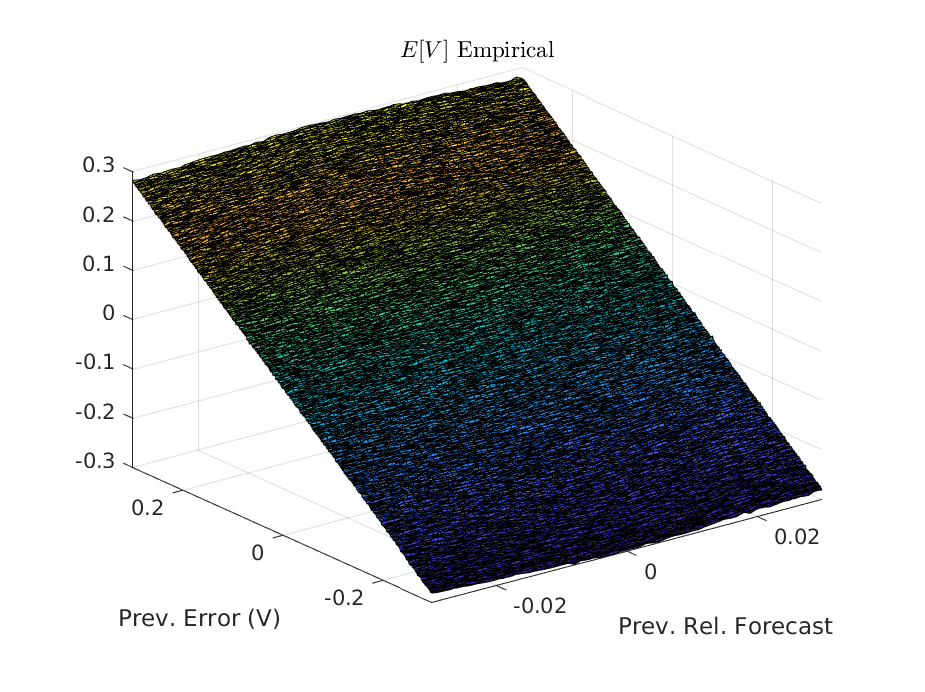
\includegraphics[width=0.48\textwidth]{../../MATLAB_Files/Results/moments/classic/1.eps}\quad
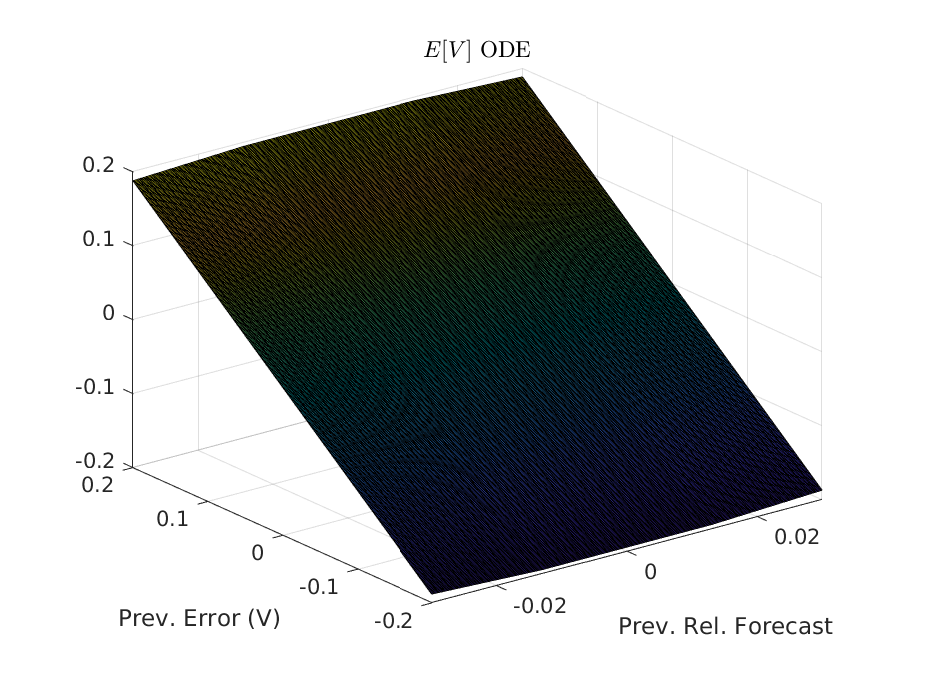
\includegraphics[width=0.48\textwidth]{../../MATLAB_Files/Results/moments/classic/2.eps}
\end{figure}

\end{frame}


\setbeamercolor{background canvas}{bg=white!10}
\begin{frame}\frametitle{Approximated first moment for $V_t$:} \label{EM1}

\begin{figure}[ht!]
\centering
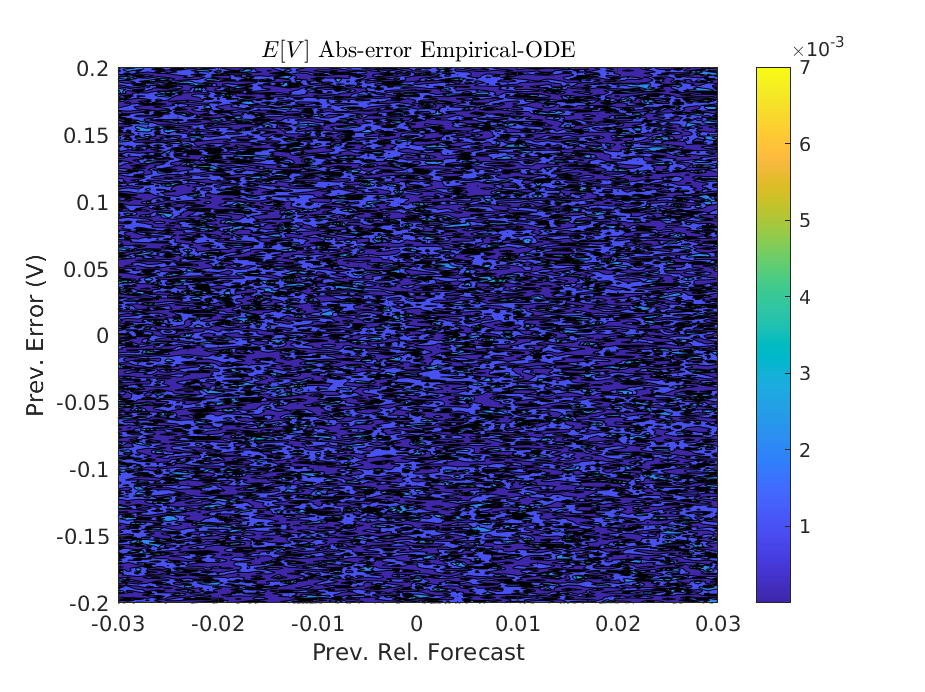
\includegraphics[width=0.48\textwidth]{../../MATLAB_Files/Results/moments/classic/3.eps}
\end{figure}

\end{frame}


\setbeamercolor{background canvas}{bg=white!10}
\begin{frame}\frametitle{Approximated second moment for $V_t$:}

\begin{figure}[ht!]
\centering
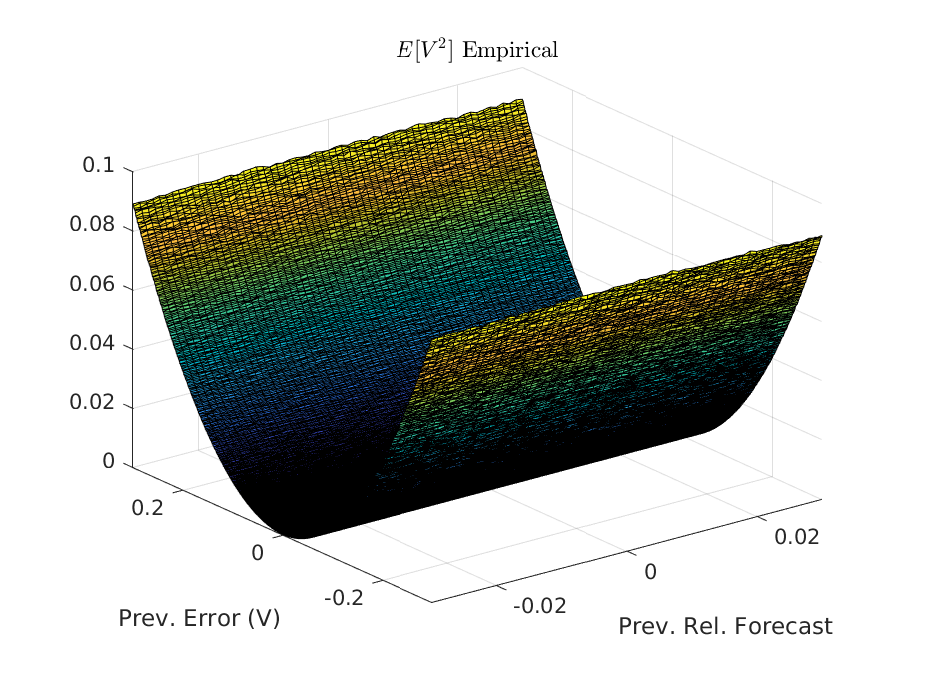
\includegraphics[width=0.48\textwidth]{../../MATLAB_Files/Results/moments/classic/4.eps}\quad
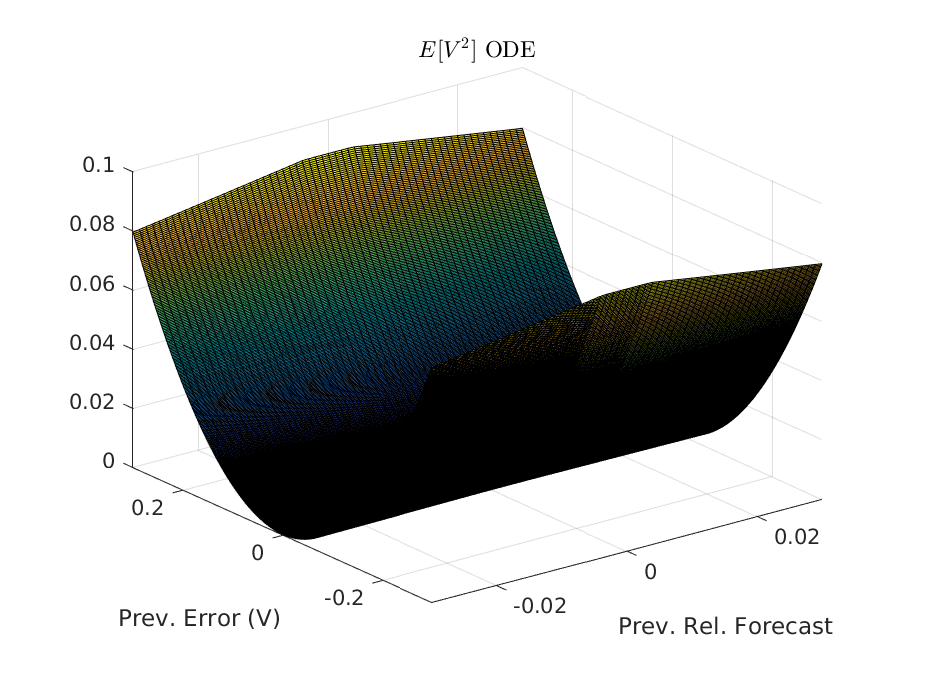
\includegraphics[width=0.48\textwidth]{../../MATLAB_Files/Results/moments/classic/5.eps}
\end{figure}

\end{frame}


\setbeamercolor{background canvas}{bg=white!10}
\begin{frame}\frametitle{Approximated second moment for $V_t$:} \label{EM2}

\begin{figure}[ht!]
\centering
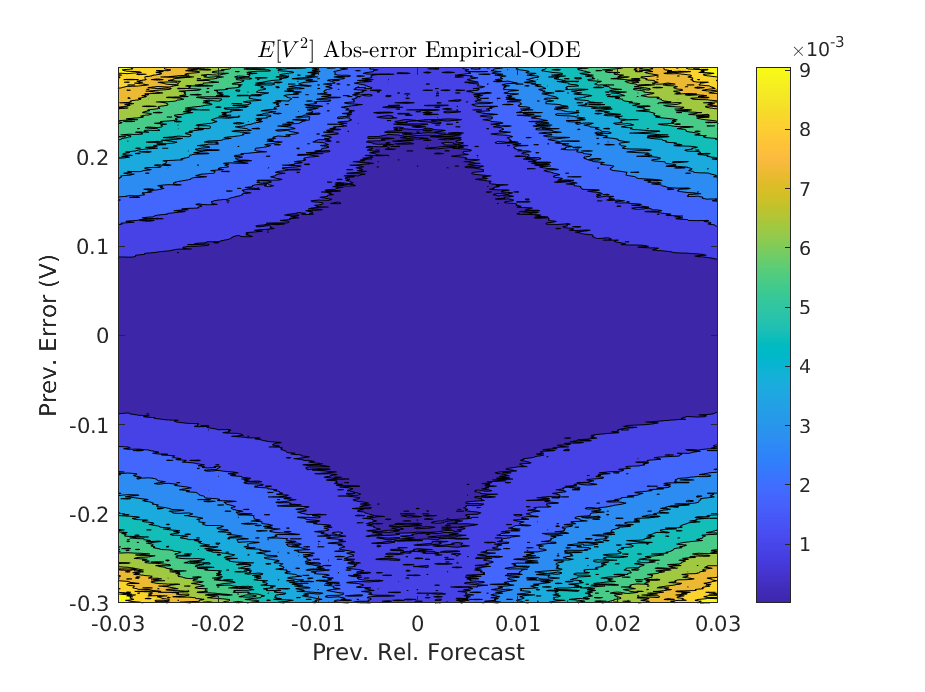
\includegraphics[width=0.48\textwidth]{../../MATLAB_Files/Results/moments/classic/6.eps}
\end{figure}

\end{frame}


\setbeamercolor{background canvas}{bg=white!10}
\begin{frame}\frametitle{Error in the moments (1/2):}

In the next plot, we sweep over the value of $p_{t_1}$ from 0.2 to 0.8 (we still fix $p_{t_1}=p_{t_2}$).\\
\quad\\
For each value of $p_{t_1}$, we repeat the procedure of slide (\ref{S1}). After we have the error matrices (see slides \ref{EM1} and \ref{EM2}), we just compute the average for each matrix. The result can be seen in the next slide.

\end{frame}


\setbeamercolor{background canvas}{bg=white!10}
\begin{frame}\frametitle{Error in the moments (2/2):}

\begin{figure}[ht!]
\centering
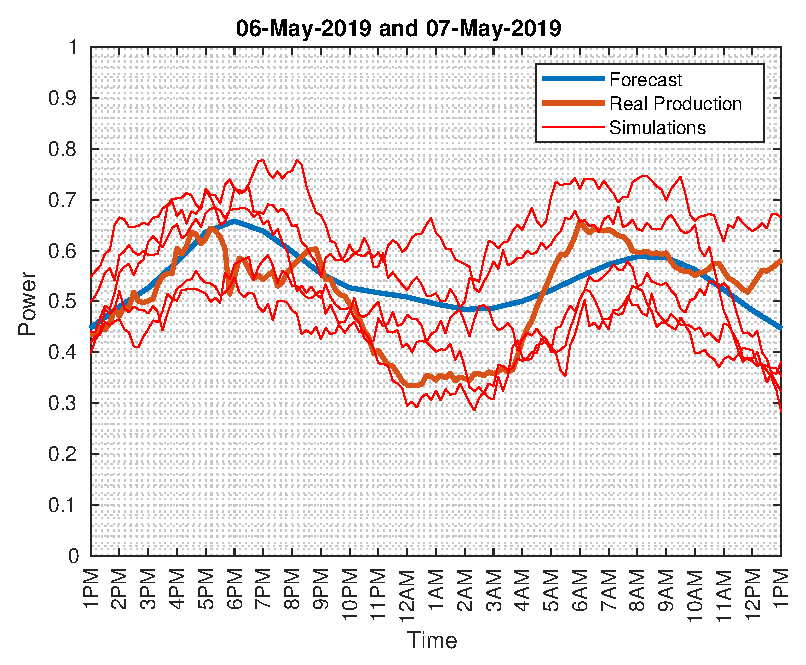
\includegraphics[width=0.48\textwidth]{../../MATLAB_Files/Results/moments/classic/7.eps}
\end{figure}

\end{frame}


\end{document}